\documentclass[hyperref={pdfpagelayout=SinglePage}]{beamer}
\usetheme{Warsaw}
\usecolortheme{default}
\usefonttheme[onlymath]{serif}
\usepackage[utf8]{inputenc}
\usepackage[spanish,activeacute]{babel}

\usepackage{graphicx}
\usepackage{fancyhdr}
\usepackage{float}
\usepackage{adjustbox}
\usepackage{subfigure}
\usepackage{amsmath}
\usepackage{ragged2e}

\usepackage{color}
\usepackage{listings}
\lstset{ %
basicstyle=\small,       % the size of the fonts that are used for the code
numbers=none,                   % where to put the line-numbers
numberstyle=\footnotesize,      % the size of the fonts that are used for the line-numbers
stepnumber=1,                   % the step between two line-numbers. If it is 1 each line will be numbered
numbersep=5pt,                  % how far the line-numbers are from the code
backgroundcolor=\color{white},  % choose the background color. You must add \usepackage{color}
showspaces=false,               % show spaces adding particular underscores
showstringspaces=false,         % underline spaces within strings
showtabs=false,                 % show tabs within strings adding particular underscores
frame=single,           % adds a frame around the code
tabsize=4,          % sets default tabsize to N spaces
captionpos=b,           % sets the caption-position to bottom
breaklines=true,        % sets automatic line breaking
breakatwhitespace=false,    % sets if automatic breaks should only happen at whitespace
escapeinside={\%*}{*)}          % if you want to add a comment within your code
}
\renewcommand{\lstlistingname}{Código}
\renewcommand\spanishtablename{Tabla}

\expandafter\def\expandafter\insertshorttitle\expandafter{%
  \insertshorttitle\hfill%
  \insertframenumber\,/\,\inserttotalframenumber}

\usepackage{animate}

\newcommand\Wider[2][5em]{%
\makebox[\linewidth][c]{%
  \begin{minipage}{\dimexpr\textwidth+#1\relax}
  \raggedright#2
  \end{minipage}%
  }%
}

\title{Dinámica Molecular regida por el paso temporal}
\subtitle{Trabajo Practico Nro. 4}
\author{Badi Leonel, Buchhalter Nicolás Demián y Meola Franco Román}
\subject{Simulación de Sistemas}
\date{\today}

\makeatletter
\@addtoreset{subfigure}{framenumber}
\makeatother

\begin{document}

\renewcommand{\figurename}{Grafico}

\begin{frame}[plain]
    \frametitle{} 
    \titlepage
    \centering
	Grupo 3
\end{frame}

\section{Fundamentos}

\subsection{Introducción}

\begin{frame}
\frametitle{Fundamentos}
\framesubtitle{Introducción}
\begin{itemize}
	\item Vamos a comparar los errores cometidos por distintos sistemas de integración
	\item Oscilador amortiguado: Sistema con sólo una partícula puntual cuya solución analítica es conocida
	\item Se implementaron:
	\begin{itemize}
		\item \textit{Beeman}
		\item \textit{Velocity Verlet}
		\item \textit{Gear Predictor Corrector de orden 5}
	\end{itemize}
\end{itemize}
\end{frame}

\subsection{Variables relevantes}

\begin{frame}
\frametitle{Fundamentos}
\framesubtitle{Variables relevantes del oscilador}
\begin{itemize}
\item Parámetros
	\begin{itemize}
		\item $m = 70$
		\item $k = 10000$
		\item $\gamma = 100$
		\item $t_{f} = 5$ 
	\end{itemize}
\item Condiciones iniciales
	\begin{itemize}
		\item $r(t=0) = 1$
		\item $v(t=0) = -\frac{2\gamma}{m}$
	\end{itemize}
\end{itemize}
\end{frame}

\section{Implementación}

\subsection{Generación de los agentes}

%\begin{frame}
%\frametitle{Implementación}
%\framesubtitle{Generación de los agentes}
%\begin{itemize}
%	\item Posiciones $(x,y)$ aleatorias para todas las partículas evitando la superposición de las mismas
%	\item $-0.1 \frac{m}{s} < v_{0} < 0.1 \frac{m}{s}$ en $x$ e $y$ para las partículas chicas
%	\item $v_{0} = 0$ para la partícula grande
%	\item Todas las paredes son rígidas
%\end{itemize}
%\end{frame}

\subsection{Simulación}

%\begin{frame}
%\frametitle{Simulación}
%\framesubtitle{Variables relevantes}
%\begin{itemize}
%	\item $dt$ intrínseco variable
%	\item $dt2$ constante
%	\item \texttt{time} : Tiempo en segundos a visualizar
%	\item $dt2 =$ \texttt{frameRate} : Número de frames por segundo
%\end{itemize}
%\end{frame}

\begin{frame}[fragile]
\frametitle{Implementación}
\framesubtitle{Cálculo Numérico}
\begin{lstlisting}[language=Java, caption = Método de Gear Predictor Corrector.]
void simulateGear(double time, double deltaT) {
	double simTime = 0;
    Oscilator oscilator = new Oscilator();
	oscilator.writePositionAndError();
    oscilator.makeEulerStep(deltaT);
    simTime += deltaT;
	oscilator.writePositionAndError();
    while (simTime < time) {
    	oscilator.makeGearStep(deltaT);
        simTime += deltaT;
		oscilator.writePositionAndError();
    }
}
\end{lstlisting}
\end{frame}

\begin{frame}
\frametitle{Implementación}
\framesubtitle{Detalles de precisión}
\begin{itemize}
	\item Todas las operaciones se realizan en \texttt{double}
	\item Se utilizan cinco cifras decimales como \texttt{output} en los archivos de salida de resultados y errores.
\end{itemize}
\end{frame}

%\subsection{Visualización}
%
%\begin{frame}
%\frametitle{Implementación}
%\framesubtitle{Visualización}
%\begin{itemize}
%	\item La simulación y la visualización son independientes
%	\item El algoritmo de simulación escribe un archivo \texttt{.tsv} con los siguientes datos:
%\begin{itemize}
%\item $(x,y)$
%\item $r$
%\item Color RGB para indicar las velocidades, donde R es la componente en el eje Y y G es la componente en eje X
%\end{itemize}
%\item Por último, se carga en \texttt{Ovito} el archivo de salida\texttt{.tsv} para realizar la visualización
%\end{itemize}
%\end{frame}

\section{Resultados}

\subsection{Tablas y Gráficos}

\begin{frame}
\frametitle{Resultados}
\framesubtitle{Error total normalizado por el número total de pasos para distintos valores de $\Delta t$}
\begin{center}
\begin{table}[h]
\centering
\adjustbox{max height=\dimexpr\textheight-3.0cm\relax,
           max width=\textwidth}{
\begin{tabular}{ccc}
\hline
\textbf{$\Delta t$} & \textbf{Método} & \textbf{$E$}\\ \hline
0.01&\textit{Beeman}&?\\
0.01&\textit{Verlet}&?\\
0.01&\textit{Gear}&?\\
0.001&\textit{Beeman}&?\\
0.001&\textit{Verlet}&?\\
0.001&\textit{Gear}&?\\
0.0001&\textit{Beeman}&?\\
0.0001&\textit{Verlet}&?\\
0.0001&\textit{Gear}&?\\
\end{tabular}
}
\caption{Suma de las diferencias al cuadrado para todos los pasos temporales normalizado por el número total de pasos}
\end{table}
\end{center}
\end{frame}

\begin{frame}
\Wider{
\frametitle{Resultados}
\framesubtitle{Gráfico de $x(t)$ para el oscilador puntual amortiguado con $\Delta t = 0.01$}
\begin{figure}[H]
        \centering
        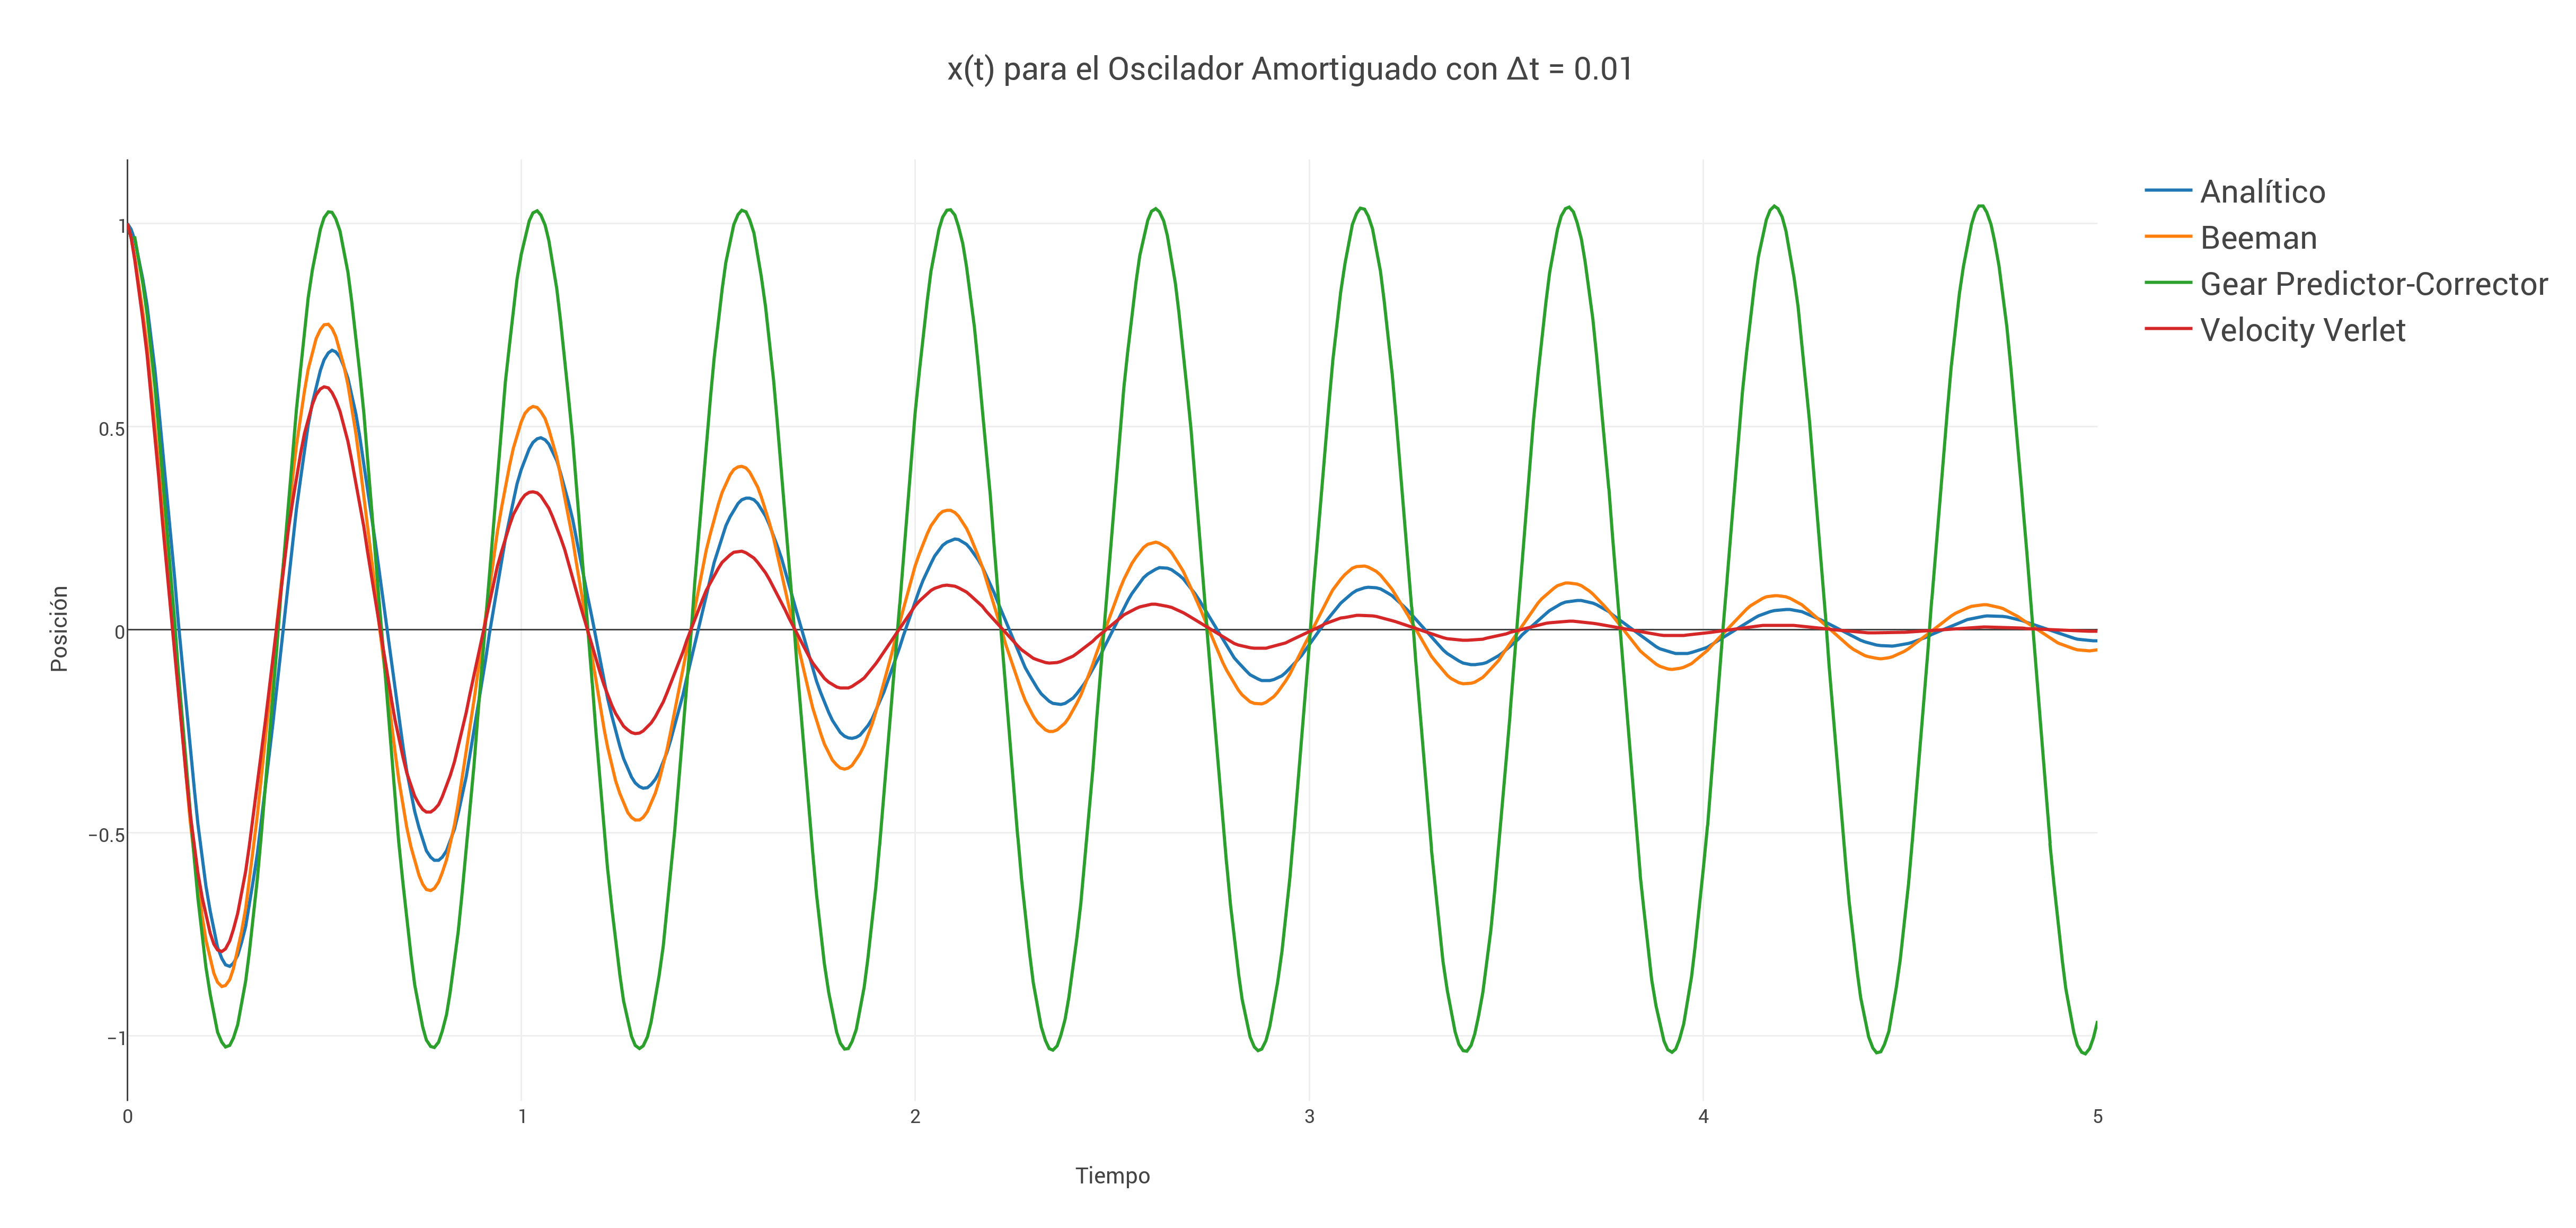
\includegraphics[width=\textwidth]{{images/0.01}.png}
\end{figure}
}
\end{frame}

\begin{frame}
\Wider{
\frametitle{Resultados}
\framesubtitle{Gráfico de $x(t)$ para el oscilador puntual amortiguado con $\Delta t = 0.001$}
\begin{figure}[H]
        \centering
        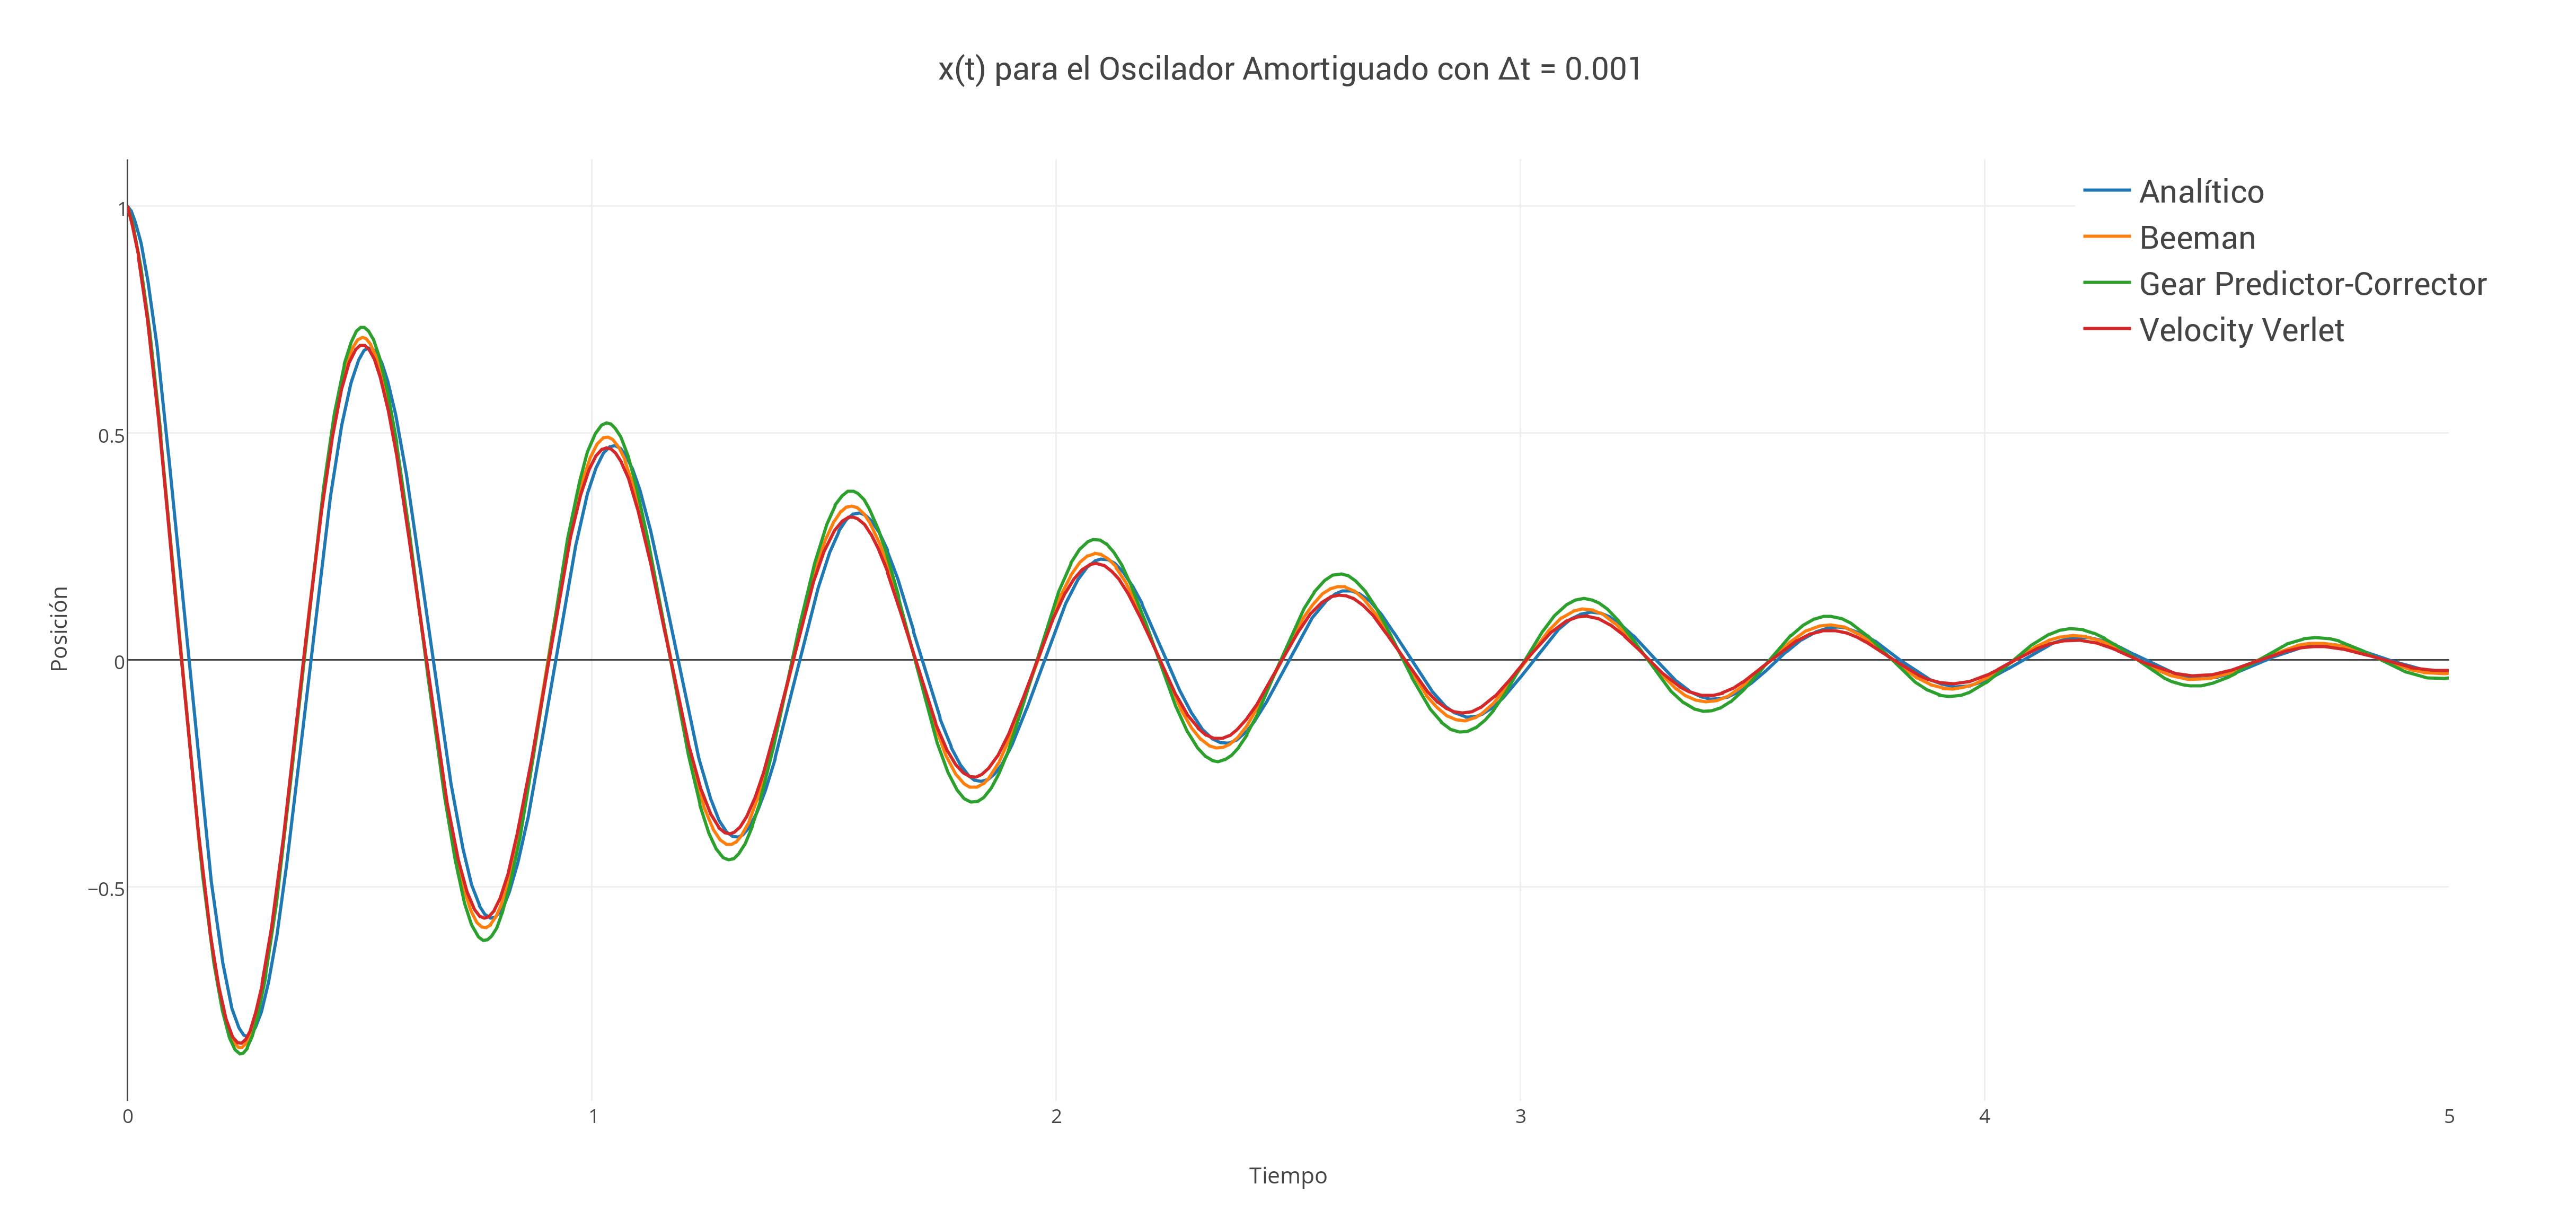
\includegraphics[width=\textwidth]{{images/0.001}.png}
\end{figure}
}
\end{frame}

\begin{frame}
\Wider{
\frametitle{Resultados}
\framesubtitle{Gráfico de $E$ para el oscilador puntual amortiguado con $\Delta t = 0.01$}
\begin{figure}[H]
        \centering
        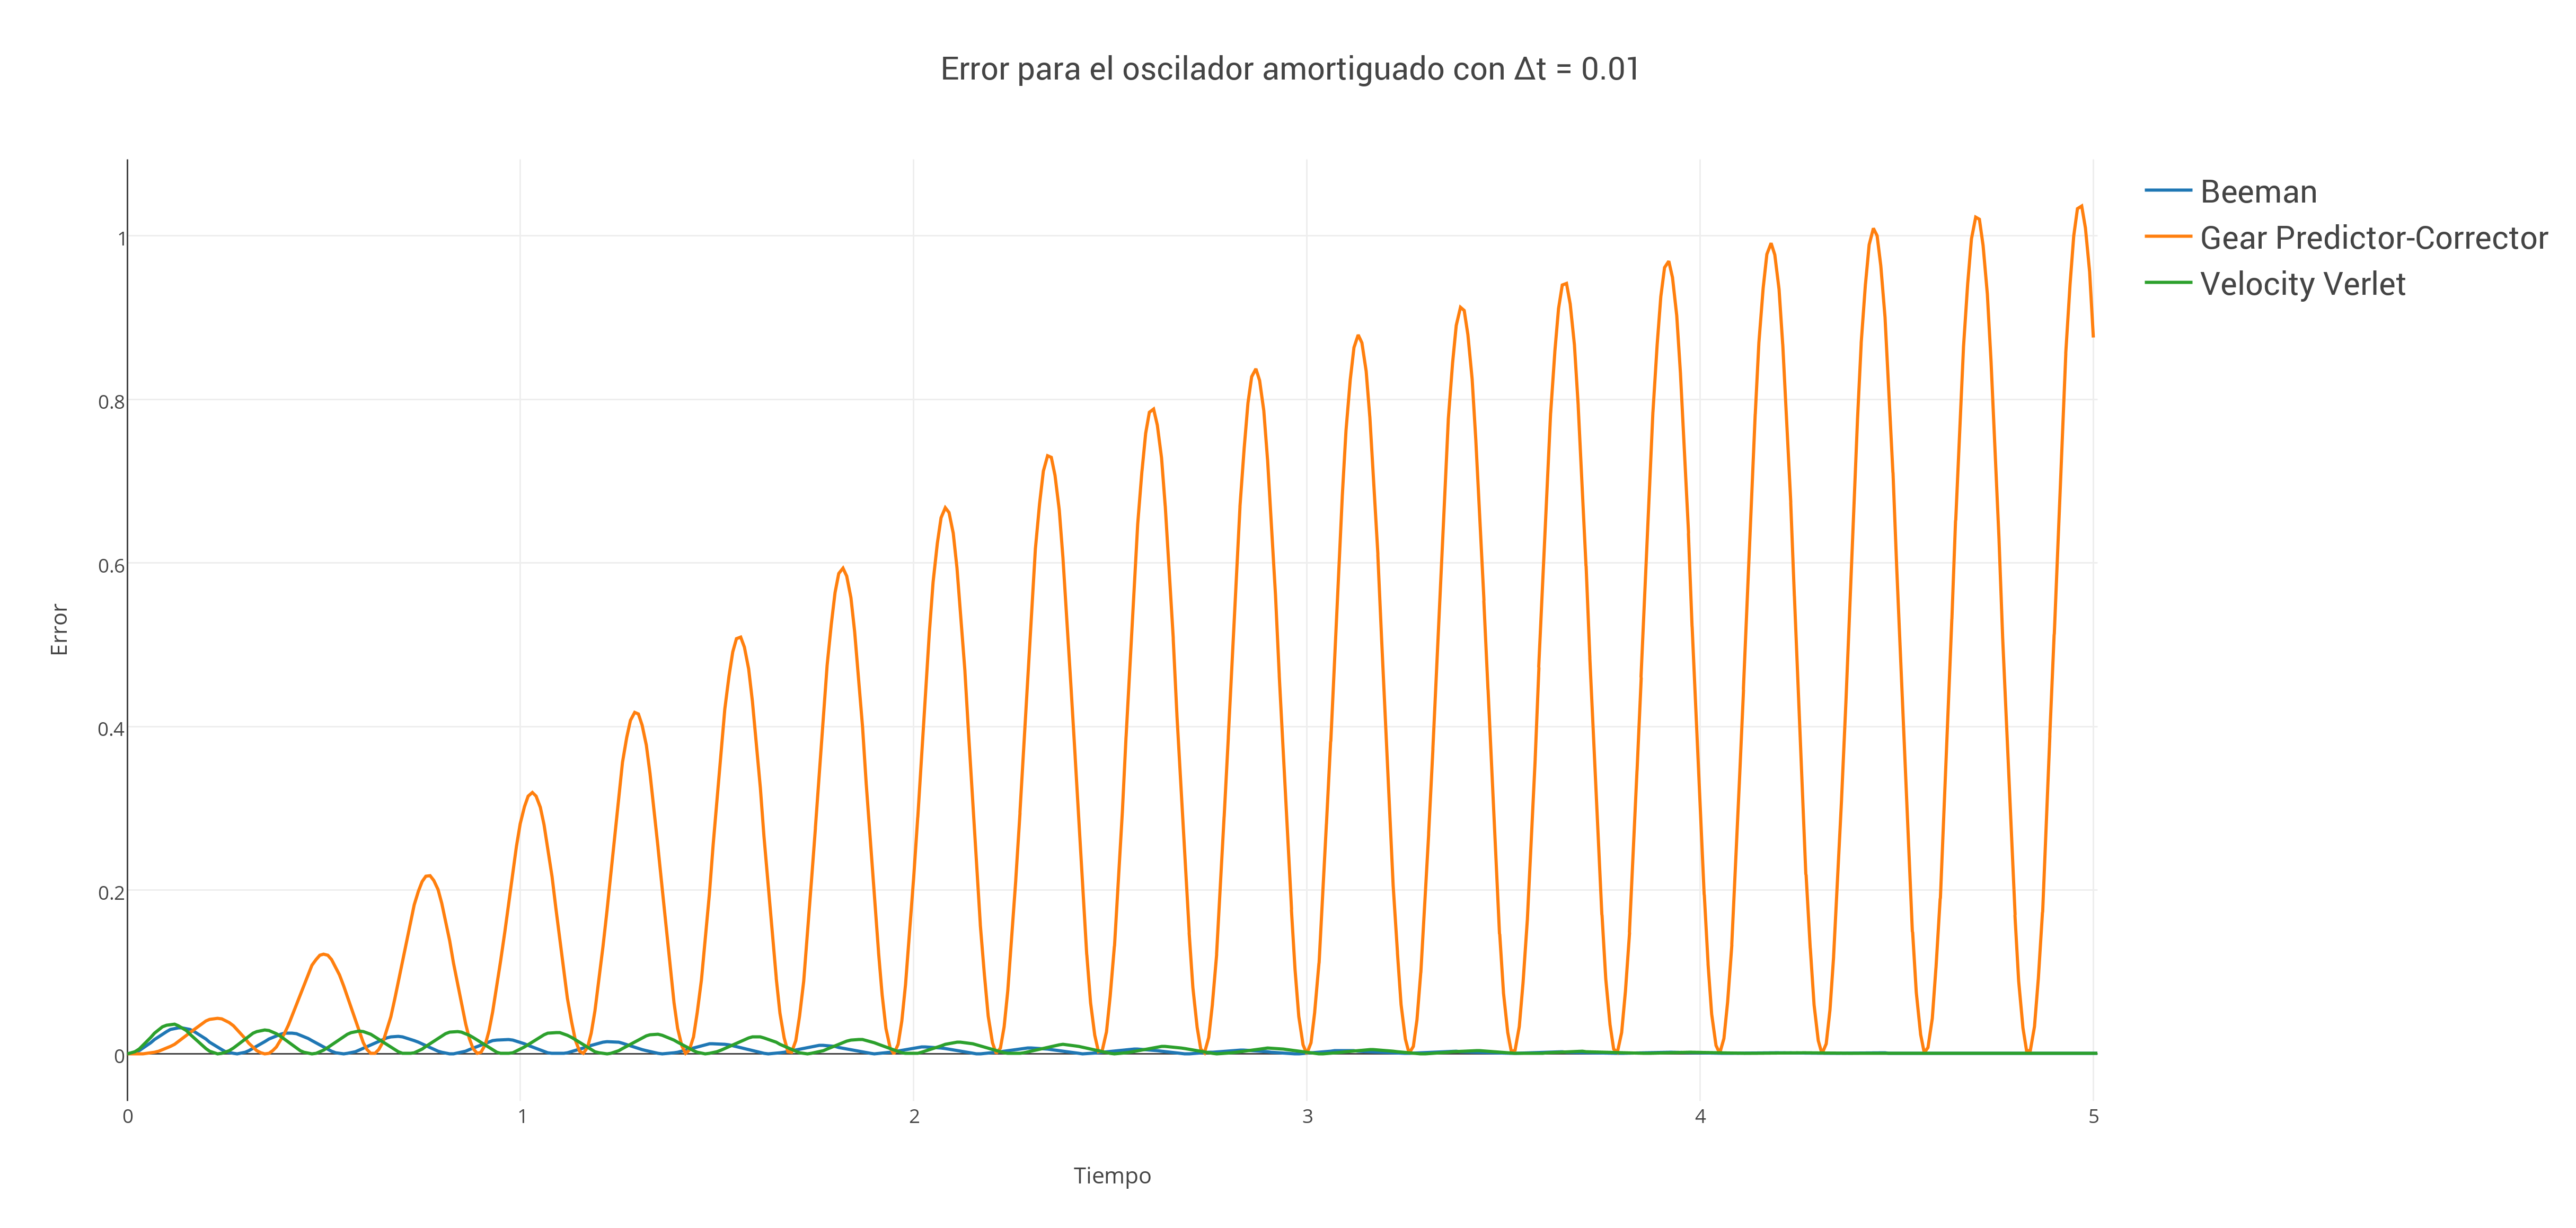
\includegraphics[width=\textwidth]{{images/Error-0.01}.png}
\end{figure}
}
\end{frame}

\begin{frame}
\Wider{
\frametitle{Resultados}
\framesubtitle{Gráfico de $E$ para el oscilador puntual amortiguado con $\Delta t = 0.001$}
\begin{figure}[H]
        \centering
        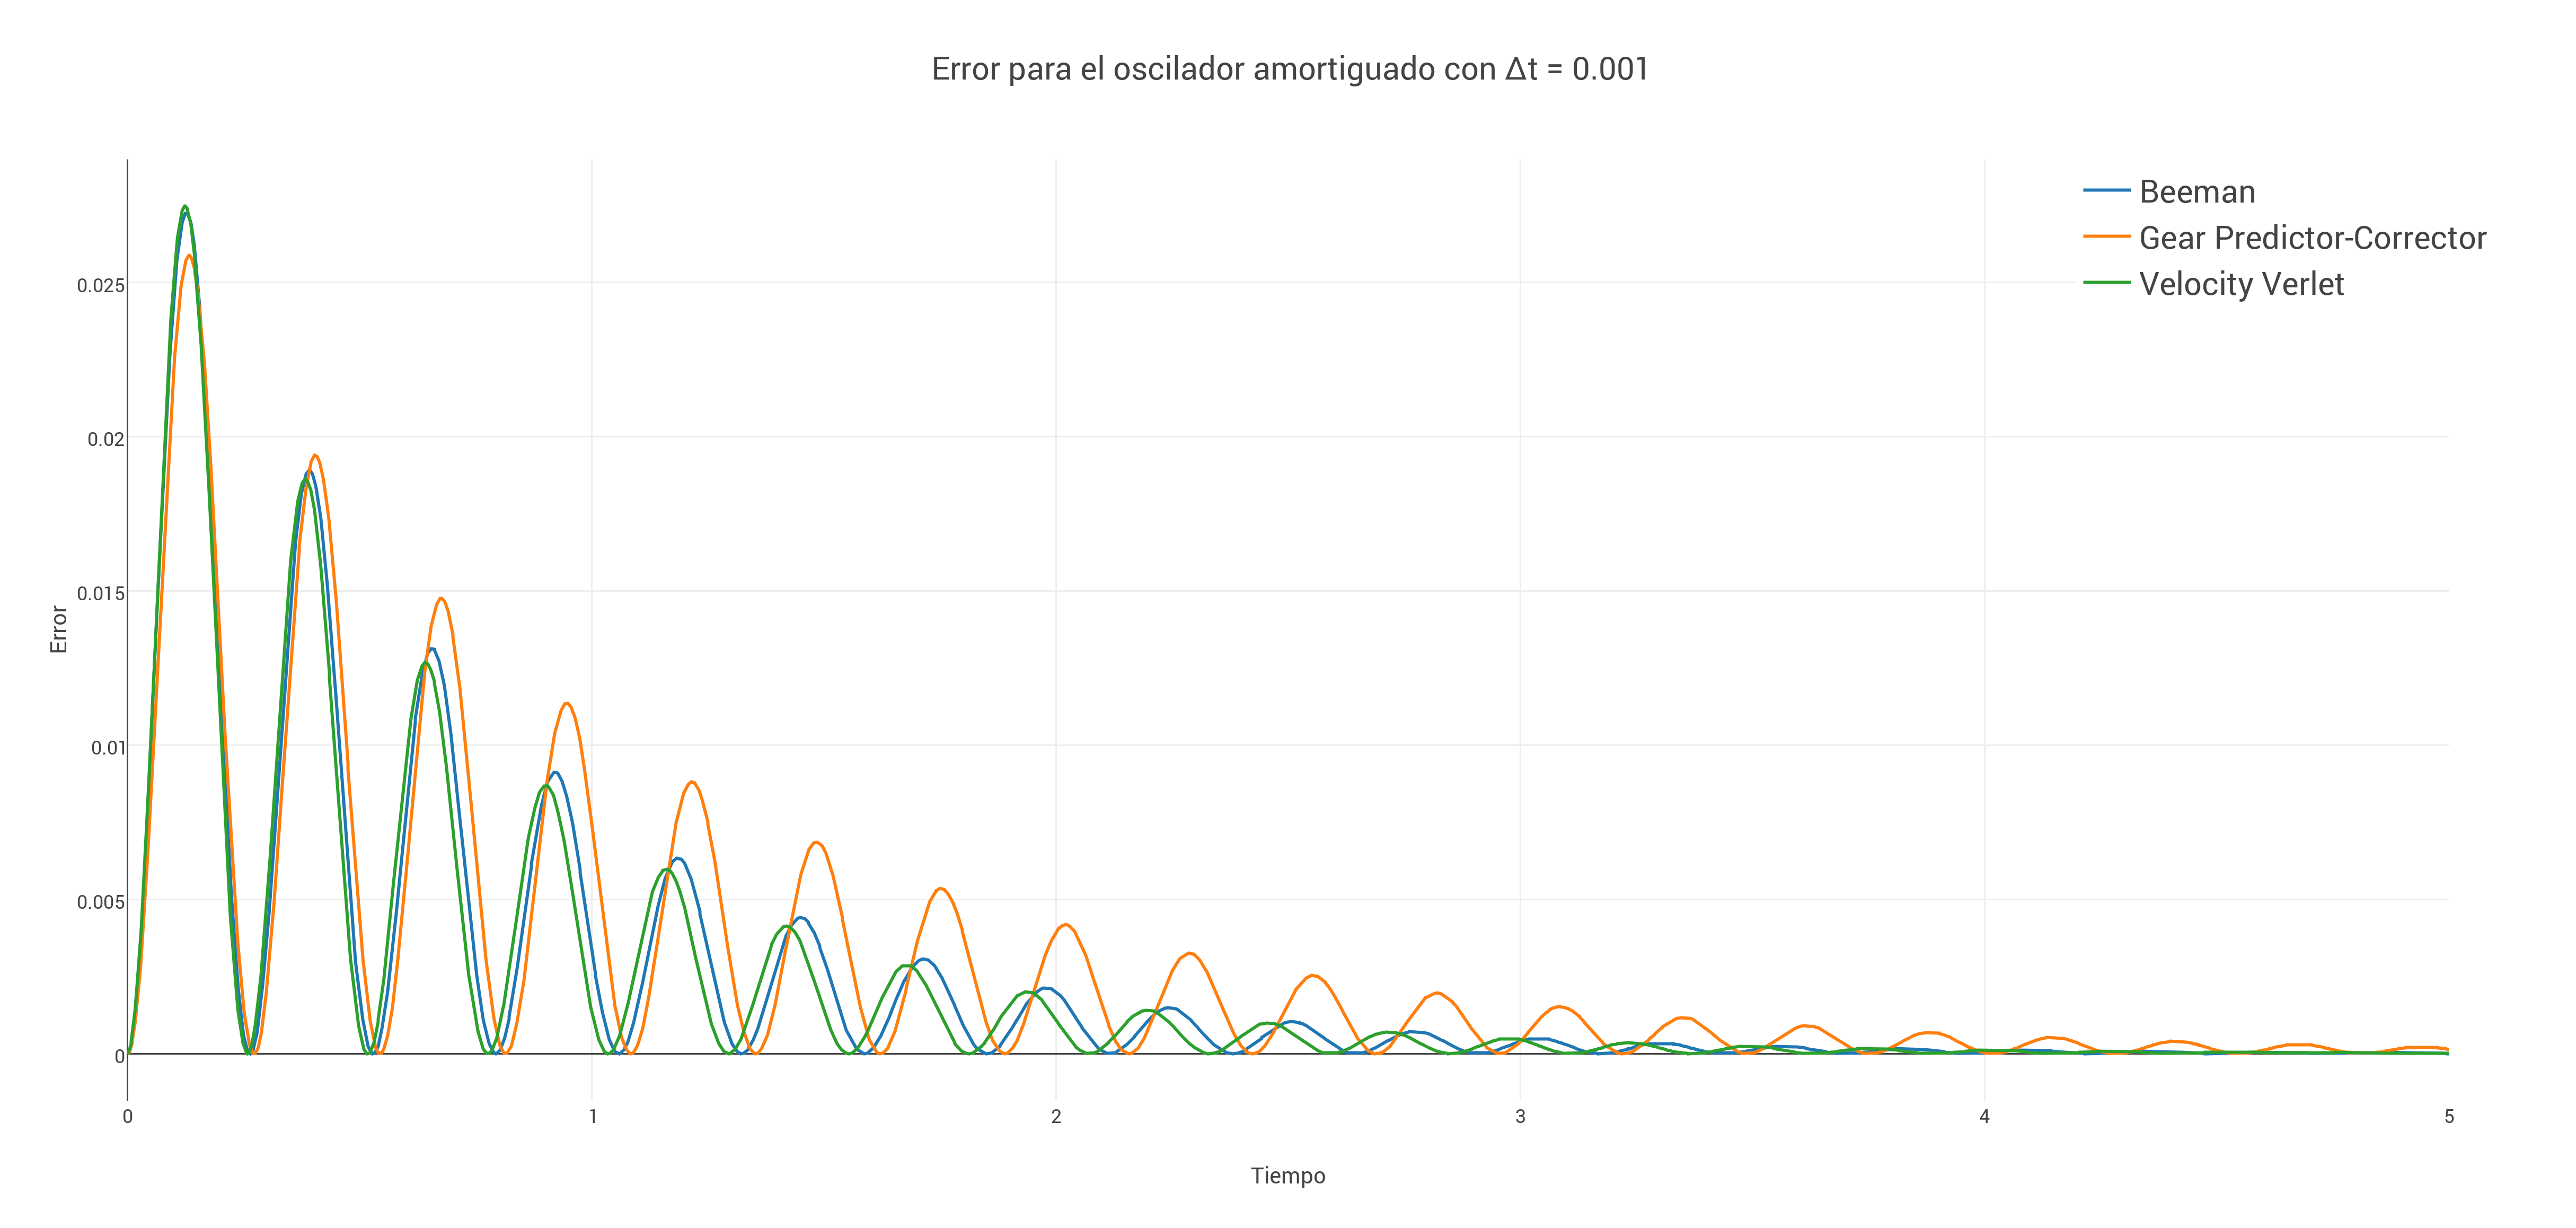
\includegraphics[width=\textwidth]{{images/Error-0.001}.png}
\end{figure}
}
\end{frame}


\subsection{Animaciones}

%\begin{frame}
%\frametitle{Resultados}
%\framesubtitle{Animación de la simulación para $N = 100$}
%\begin{figure}[H]
%	\centering
%	\animategraphics[loop,controls,width=0.75\textheight]{10}{animation/dmer-100-}{0000}{0200}
%\end{figure}
%\end{frame}
%
%\begin{frame}
%\frametitle{Resultados}
%\framesubtitle{Animación de la simulación para $N = 500$}
%\begin{figure}[H]
%	\centering
%	\animategraphics[loop,controls,width=0.75\textheight]{10}{animation/dmer-500-}{0000}{0200}
%\end{figure}
%\end{frame}
%
%\begin{frame}
%\frametitle{Resultados}
%\framesubtitle{Animación de la simulación para $N = 1000$}
%\begin{figure}[H]
%	\centering
%	\animategraphics[loop,controls,width=0.75\textheight]{10}{animation/dmer1000-}{0000}{0200}
%\end{figure}
%\end{frame}

\subsection{Conclusiones}

\begin{frame}
\frametitle{Conclusiones}
\begin{itemize}
	\item Con un $\Delta t = 0.001$ obtuvimos resultados con errores muy bajos para los tres métodos.	
	\item \textit{Gear Predictor-Corrector} es el que dio peores resultados para el caso puntual.
	\item Para una cantidad de pasos baja ($\Delta t = 0.001$), el error de \textit{Gear Predictor-Corrector} aumenta, simulando un oscilador que no disipa energía.
	\item Las diferencias de los errores entre \textit{Beeman} y \textit{Velocity Verlet} son menores.
	\item \textbf{El esquema de integración que resulta mejor para este sistema es ?}.
	\end{itemize}	
\end{frame}

\begin{frame}[plain,c]
\begin{center}
	\Huge Gracias
\end{center}
\end{frame}

\end{document}